
% Options for packages loaded elsewhere
\PassOptionsToPackage{unicode}{hyperref}
\PassOptionsToPackage{hyphens}{url}
\documentclass[]{report}
\usepackage{xcolor}
\usepackage{amsmath,amssymb}
\setcounter{secnumdepth}{5}
\usepackage{iftex}
\usepackage[T1]{fontenc}
\usepackage[utf8]{inputenc}
\usepackage{textcomp} % provide euro and other symbols
\usepackage[]{fontawesome}

% Use upquote if available, for straight quotes in verbatim environments
\IfFileExists{upquote.sty}{\usepackage{upquote}}{}
\IfFileExists{microtype.sty}{% use microtype if available
  \usepackage[]{microtype}
  \UseMicrotypeSet[protrusion]{basicmath} % disable protrusion for tt fonts
}{}
\makeatletter
\@ifundefined{KOMAClassName}{% if non-KOMA class
  \IfFileExists{parskip.sty}{%
    \usepackage{parskip}
  }{% else
    \setlength{\parindent}{0pt}
    \setlength{\parskip}{6pt plus 2pt minus 1pt}}
}{% if KOMA class
  \KOMAoptions{parskip=half}}
\makeatother
\setlength{\emergencystretch}{3em} % prevent overfull lines
\providecommand{\tightlist}{%
  \setlength{\itemsep}{0pt}\setlength{\parskip}{0pt}}
\usepackage[explicit]{titlesec}
\usepackage[svgnames]{xcolor}
\usepackage{enumitem}
\usepackage{multirow}
\usepackage{array}
\usepackage{calc}
\usepackage{layouts}
\usepackage{pdfpages}

% section headers
\titlespacing{\chapter}{0pt}{0pt}{0pt}

\titleformat{\chapter}
  [hang]
  {\normalfont\sffamily\Large\color{white}}
  {}
  {0.5ex}
  {\colorbox{Navy}{\makebox[4em][l]{Article \thechapter} \makebox[\textwidth - 5em][l]{#1} }}  
  %{\colorbox{RoyalBlue}{%
  %  \begin{tabular}{ p{11em} p{\textwidth - 10em} }
  %    Article \thechapter & #1 \\
  %  \end{tabular}
  %}}

% \newcommand{\chapterbreak}{\addpenalty{-500}\vspace*{0pt}}

\titleformat{\section}
  {\normalfont\sffamily}
  {}
  {0.5ex}
  {#1}

% enumerations
\renewcommand{\labelenumi}{\arabic{enumi}}
\renewcommand{\labelenumii}{\arabic{enumi}.\arabic{enumii}}
\renewcommand{\labelenumiii}{\arabic{enumi}.\arabic{enumii}.\arabic{enumiii}}
\renewcommand{\labelenumiv}{\arabic{enumi}.\arabic{enumii}.\arabic{enumiii}.\arabic{enumiv}}

\setlist[enumerate,1]{leftmargin=3ex, rightmargin=0pt, topsep=0pt,%
                       labelsep=1ex, listparindent=0pt, itemsep=1ex}
\setlist[enumerate,2]{leftmargin=4ex, rightmargin=0pt, labelsep=1ex, labelwidth=0em}
\setlist[enumerate,3]{leftmargin=6ex, rightmargin=0pt, labelsep=1ex, labelwidth=0em}
% \setlength{\listparindent=0pt},

% environment for the explanations
\newenvironment{expl}[0]%
  {\rule{\textwidth}{.2pt}\footnotesize}%
  {\rule{\textwidth}{.2pt}\normalsize}



\usepackage{bookmark}
\IfFileExists{xurl.sty}{\usepackage{xurl}}{} % add URL line breaks if available
\urlstyle{same}
\hypersetup{
  hidelinks,
  pdfcreator={LaTeX via pandoc}}

\author{}
\date{}


\begin{document}

\chapter{Purpose}

\begin{enumerate}
\tightlist
\item
\input{1.1.txt}
\end{enumerate}

\begin{expl}
\section{(Interpretation)}\label{interpretation}
\input{1.i_1.txt}
\end{expl}

\chapter{Application}\label{application}

\begin{enumerate}
\item
\input{2.1.txt}
\item
\input{2.2.txt}
\item
\input{2.3.txt}
\end{enumerate}

\begin{expl}
\section{(Explanation\#1)}\label{explanation1}
\input{2.e_1.txt}
\end{expl}


\chapter{Competition Area}\label{competition-area}

\begin{enumerate}
\item
\input{3.1.txt}
  \begin{enumerate}
  \item
  \input{3.1.1.txt}
  \item
  \input{3.1.2.txt}
  \end{enumerate}
\item
\input{3.2.txt}
  \begin{enumerate}
  \item
  \input{3.2.1.txt}
  \item
  \input{3.2.2.txt}
  \item
  \input{3.2.3.txt}
  \item
  \input{3.2.4.txt}
  \item
  \input{3.2.5.txt}
  \item
  \input{3.2.6.txt}
  \item
  \input{3.2.7.txt}
  \end{enumerate}
\item
\input{3.3.txt}
  \begin{itemize}
  \tightlist
  \item
  \input{3.3.1.txt}
  \item
  \input{3.3.2.txt}
  \item
  \input{3.3.3.txt}
  \item
  \input{3.3.4.txt}
  \end{itemize}
\end{enumerate}

\begin{expl}
\section{(Explanation \#1)}\label{explanation-1}
\input{3.e_1.txt}

\section{(Explanation \#2)}\label{explanation-2}
\input{3.e_2.txt}

\section{(Explanation \#3)}\label{explanation-3}
\input{3.e_3.txt}
\end{expl}

%todo: Ide kell a rajz!
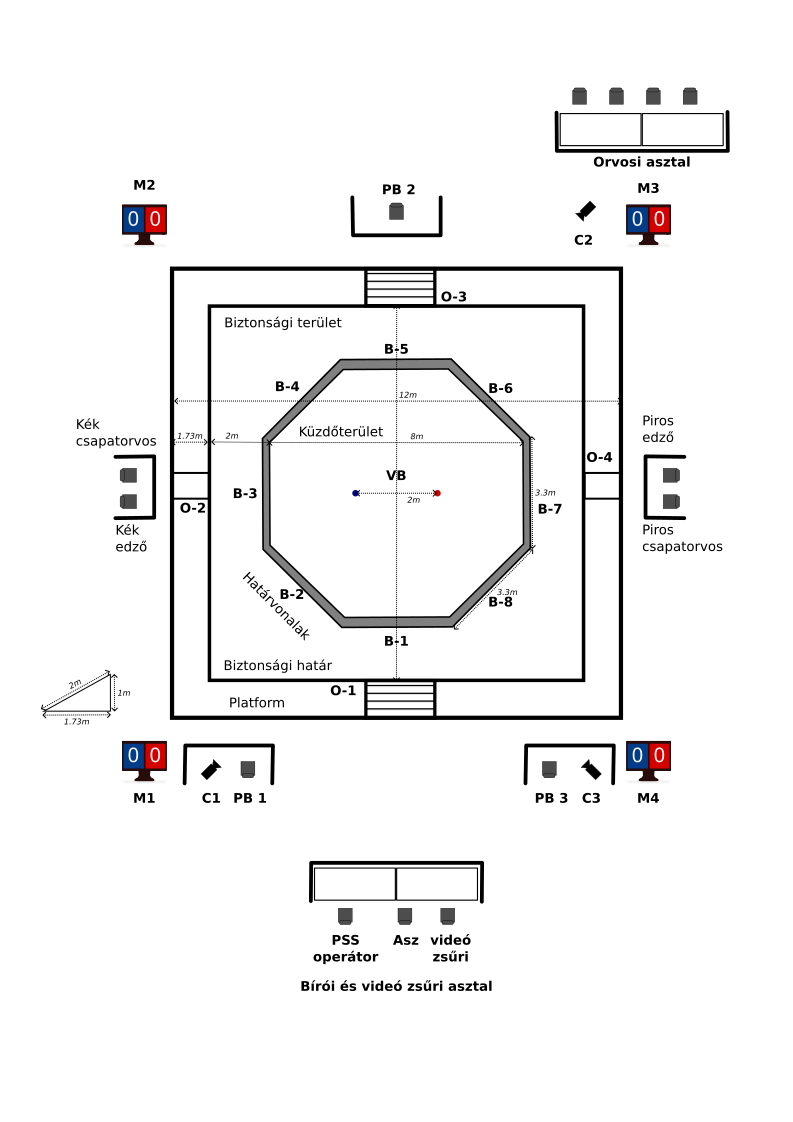
\includepdf{octogon_on_platform.pdf}
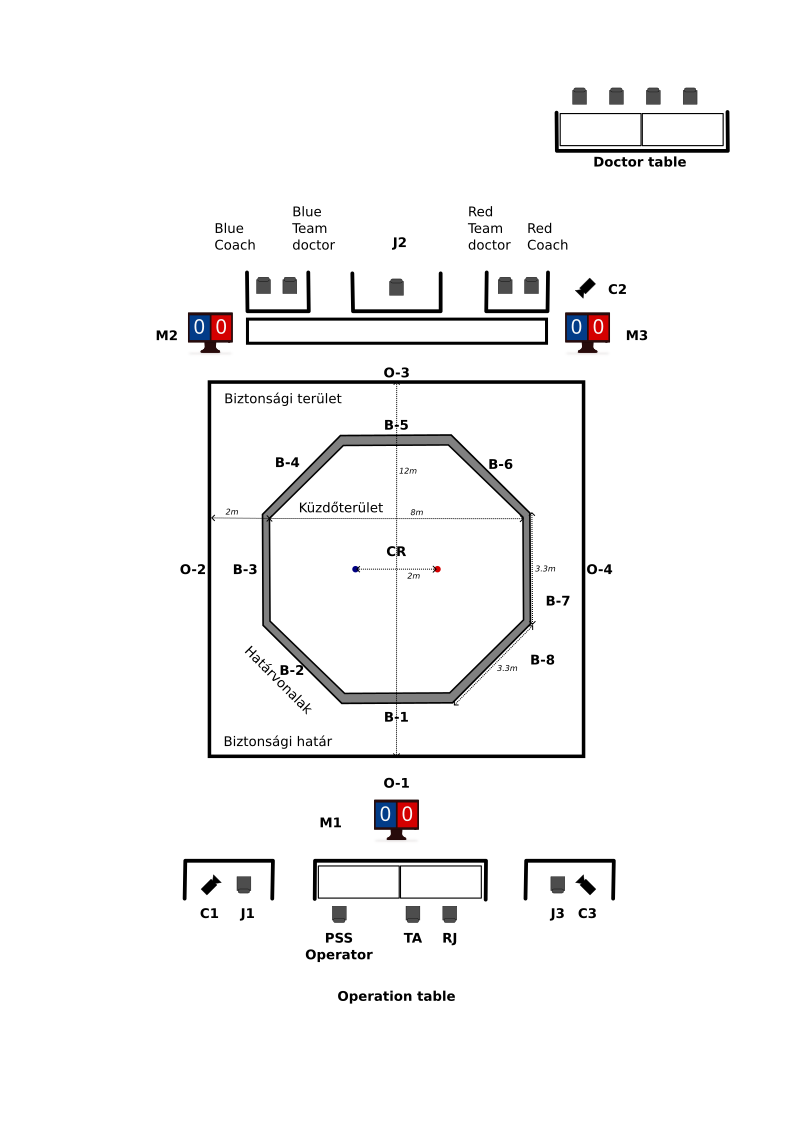
\includepdf{octogon_on_floor.pdf}
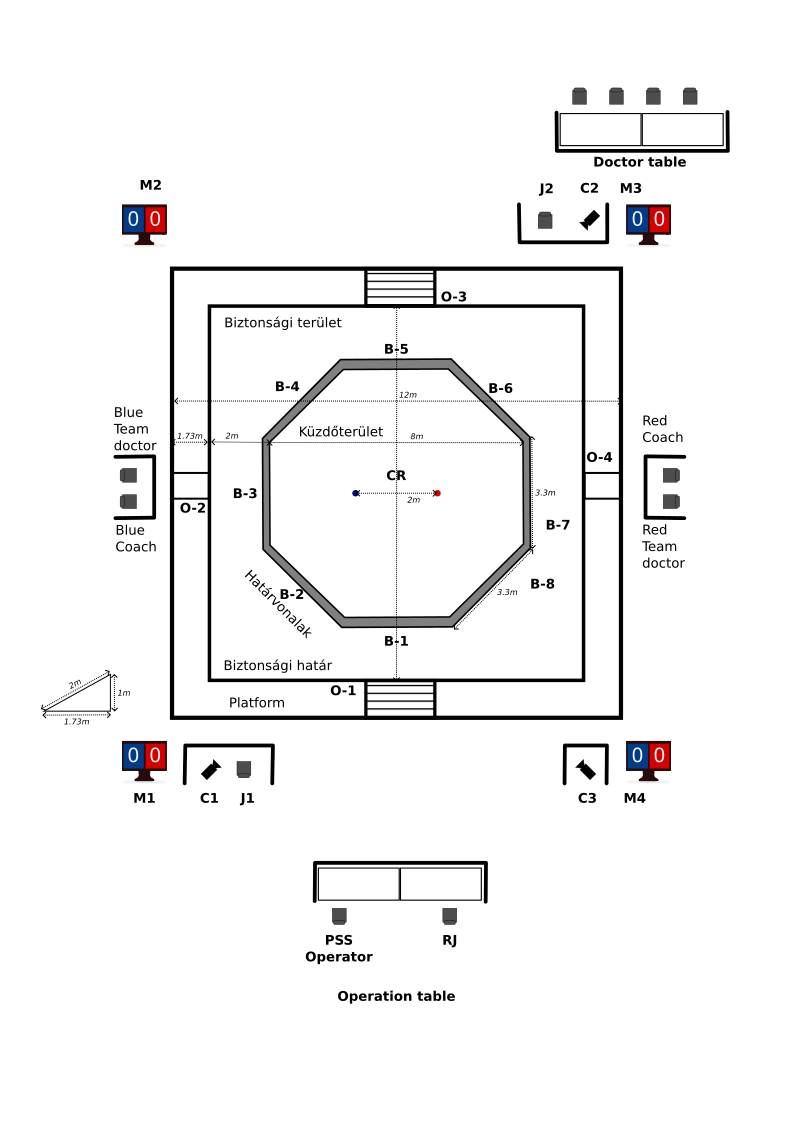
\includepdf{octogon_on_platform_2_judges.pdf}
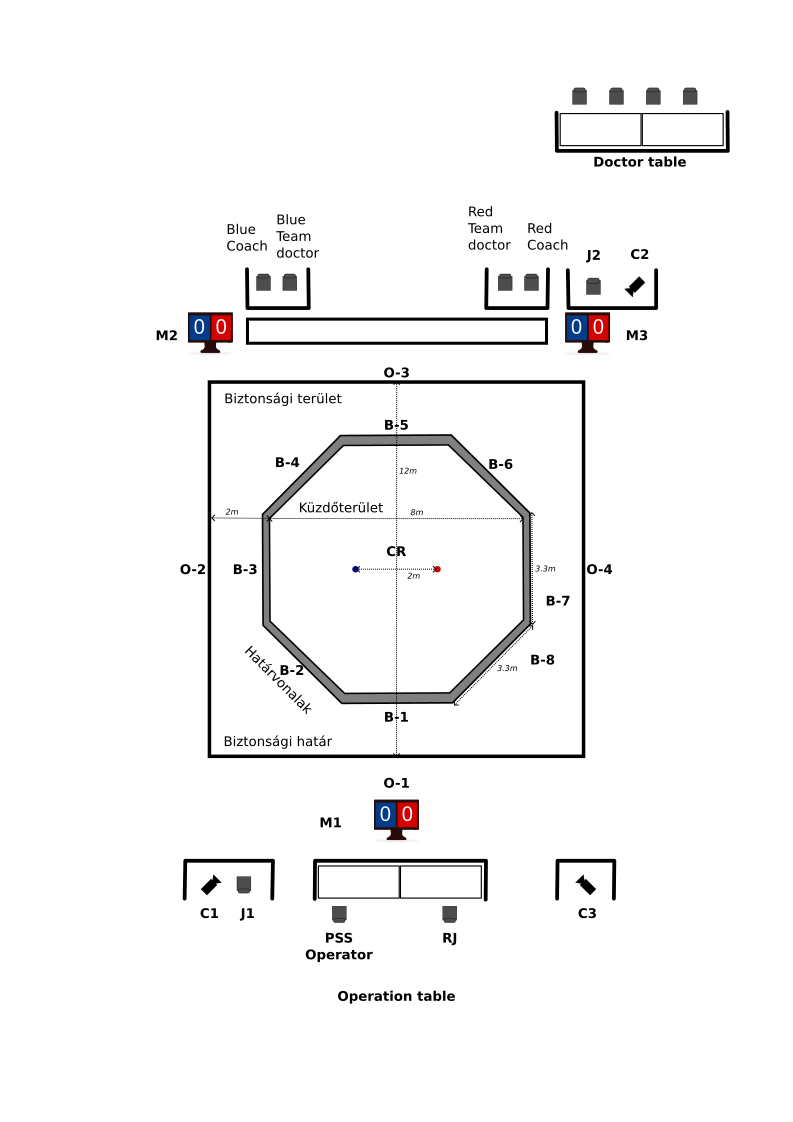
\includepdf{octogon_on_floor_2_judges.pdf}


\chapter{Contestant}\label{contestant}

\begin{enumerate}
\item
\input{4.1.txt}

  \begin{enumerate}
  \item
  \input{4.1.1.txt}
  \item
  \input{4.1.2.txt}
  \item
  \input{4.1.3.txt}
  \item
  \input{4.1.4.txt}
  \item
  \input{4.1.5.txt}
  \end{enumerate}
\end{enumerate}

\begin{expl}
\section{(Interpretation)}\label{interpretation-1}
\input{4.i_1.txt}

\section{(Interpretation)}\label{interpretation-2}
\input{4.i_2.txt}

\section{(Interpretation)}\label{interpretation-3}
\input{4.i_3.txt}
\end{expl}

\begin{enumerate}[resume*]
\item
\input{4.2.txt}

  \begin{enumerate}
  \item
  \input{4.2.1.txt}

    \begin{enumerate}
    \item
    \input{4.2.1.1.txt}
    \end{enumerate}

  \item
  \input{4.2.2.txt}
  \item
  \input{4.2.3.txt}
  \item
  \input{4.2.4.txt}
  \item
  \input{4.2.5.txt}

    \begin{enumerate}
    \item
    \input{4.2.5.1.txt}

    \item
    \input{4.2.5.2.txt}
    \item
    \input{4.2.5.3.txt}
    \end{enumerate}

  \end{enumerate}

\item
\input{4.3.txt}

  \begin{enumerate}
  \item
  \input{4.3.1.txt}
  \item
  \input{4.3.2.txt}
  \item
  \input{4.3.3.txt}
  \item
  \input{4.3.4.txt}
  \end{enumerate}

\end{enumerate}

\begin{expl}
\section{(Explanation \#1)}\label{explanation-1-1}
\input{4.i_1.txt}

\section{(Explanation \#2)}\label{explanation-2-1}
\input{4.i_2.txt}

\section{(Explanation \#3)}\label{explanation-3-1}
\input{4.e_3.txt}

\section{(Explanation \#4)}\label{explanation-4}
\input{4.e_4.txt}

\section{(Explanation \#5)}\label{explanation-5}
\input{4.e_5.txt}

\section{(Explanation \#6)}\label{explanation-6}
\input{4.e_6.txt}

\section{(Explanation \#7)}\label{explanation-7}
\input{4.e_7.txt}

\section{(Explanation \#8)}\label{explanation-8}
\input{4.e_8.txt}

\section{(Explanation \#9)}\label{explanation-9}
\input{4.e_9.txt}

\section{(Explanation \#10)}\label{explanation-10}
\input{4.e_10.txt}
\end{expl}


\chapter{Weight category}\label{weight-category}

\begin{enumerate}

\item
\input{5.1.txt}

\begin{center}
\begin{tabular}{ |l|l|l|l| } 
 \hline
 \multicolumn{2}{|l|}{Men's division} & \multicolumn{2}{|l|}{Women's division}  \\
 \hline
 Under 54 kg & Not exceeding 54 kg & under 46 kg & Not exceeding 46 kg \\
 \hline
 Under 58 kg & Over 54 kg \& Not exceeding 58 kg & Under 49 kg & Over 46 kg \& Not exceeding 49 kg \\
 \hline
 Under 63 kg & Over 58 kg \& Not exceeding 63 kg & Under 53 kg & Over 49 kg \& Not exceeding 53 kg \\
 \hline
 Under 68 kg & Over 63 kg \& Not exceeding 68 kg & Under 57 kg & Over 53 kg \& Not exceeding 57 kg \\
 \hline
 Under 74 kg & Over 68 kg \& Not exceeding 74 kg & Under 62 kg & Over 57 kg \& Not exceeding 62 kg \\
 \hline
 Under 80 kg & Over 74 kg \& Not exceeding 80 kg & Under 67 kg & Over 62 kg \& Not exceeding 67 kg \\
 \hline
 Under 87 kg & Over 80 kg \& Not exceeding 87 kg & Under 73 kg & Over 67 kg \& Not exceeding 73 kg \\
 \hline
 Over 87 kg & Over 54 kg \& Not exceeding 58 kg & Over 73 kg & Over 73 kg \\
 \hline
\end{tabular}
\end{center}

\item
\input{5.2.txt}

\begin{center}
\begin{tabular}{ |l|l|l|l| } 
 \hline
 \multicolumn{2}{|l|}{Men's division} & \multicolumn{2}{|l|}{Women's division}  \\
 \hline
 Under 58 kg & Not exceeding 58 kg & under 49 kg & Not exceeding 49 kg \\
 \hline
 Under 68 kg & Over 58 kg \& Not exceeding 68 kg & Under 57 kg & Over 49 kg \& Not exceeding 57 kg \\
 \hline
 Under 80 kg & Over 68 kg \& Not exceeding 80 kg & Under 67 kg & Over 57 kg \& Not exceeding 67 kg \\
 \hline
 Over 80 kg & Over 50 kg & Over 67 kg & Over 67 kg \\
 \hline
\end{tabular}
\end{center}

\begin{samepage}
\item
\input{5.3.txt}

\begin{center}
\begin{tabular}{ |l|l|l|l| } 
 \hline
 \multicolumn{2}{|l|}{Men's division} & \multicolumn{2}{|l|}{Women's division}  \\
 \hline
 Under 45 kg & Not exceeding 45 kg & under 42 kg & Not exceeding 42 kg \\
 \hline
 Under 48 kg & Over 45 kg \& Not exceeding 44 kg & Under 49 kg & Over 42 kg \& Not exceeding 44 kg \\
 \hline
 Under 51 kg & Over 48 kg \& Not exceeding 46 kg & Under 53 kg & Over 44 kg \& Not exceeding 46 kg \\
 \hline
 Under 55 kg & Over 51 kg \& Not exceeding 49 kg & Under 49 kg & Over 46 kg \& Not exceeding 49 kg \\
 \hline
 Under 59 kg & Over 55 kg \& Not exceeding 52 kg & Under 53 kg & Over 49 kg \& Not exceeding 52 kg \\
 \hline
 Under 63 kg & Over 59 kg \& Not exceeding 55 kg & Under 57 kg & Over 52 kg \& Not exceeding 55 kg \\
 \hline
 Under 68 kg & Over 63 kg \& Not exceeding 59 kg & Under 62 kg & Over 55 kg \& Not exceeding 59 kg \\
 \hline
 Under 73 kg & Over 68 kg \& Not exceeding 63 kg & Under 67 kg & Over 69 kg \& Not exceeding 63 kg \\
 \hline
 Under 78 kg & Over 73 kg \& Not exceeding 68 kg & Under 73 kg & Over 63 kg \& Not exceeding 68 kg \\
 \hline
 Over 78 kg & Over 78 kg \& Not exceeding 58 kg & Over 68 kg & Over 68 kg \\
 \hline
\end{tabular}
\end{center}
\end{samepage}

\item
\input{5.4.txt}

\begin{center}
\begin{tabular}{ |l|l|l|l| } 
 \hline
 \multicolumn{2}{|l|}{Men's division} & \multicolumn{2}{|l|}{Women's division}  \\
 \hline
 Under 48 kg & Not exceeding 48 kg & under 44 kg & Not exceeding 44 kg \\
 \hline
 Under 55 kg & Over 48 kg \& Not exceeding 55 kg & Under 49 kg & Over 44 kg \& Not exceeding 49 kg \\
 \hline
 Under 63 kg & Over 55 kg \& Not exceeding 63 kg & Under 55 kg & Over 49 kg \& Not exceeding 55 kg \\
 \hline
 Under 73 kg & Over 65 kg \& Not exceeding 73 kg & Under 63 kg & Over 55 kg \& Not exceeding 63 kg \\
 \hline
 Over 73 kg & Over 73 kg & Over 63 kg & Over 63 kg \\
 \hline
\end{tabular}
\end{center}

\item
\input{5.5.txt}

\begin{center}
\begin{tabular}{ |l|l|l|l| } 
 \hline
 \multicolumn{2}{|l|}{Men's division} & \multicolumn{2}{|l|}{Women's division}  \\
 \hline
 Under 33 kg & Not exceeding 33 kg & under 29 kg & Not exceeding 29 kg \\
 \hline
 Under 37 kg & Over 33 kg \& Not exceeding 37 kg & Under 33 kg & Over 29 kg \& Not exceeding 33 kg \\
 \hline                                                                                        
 Under 41 kg & Over 37 kg \& Not exceeding 41 kg & Under 37 kg & Over 33 kg \& Not exceeding 37 kg \\
 \hline                                                                                        
 Under 45 kg & Over 41 kg \& Not exceeding 45 kg & Under 41 kg & Over 37 kg \& Not exceeding 41 kg \\
 \hline                                                                                        
 Under 49 kg & Over 45 kg \& Not exceeding 49 kg & Under 44 kg & Over 41 kg \& Not exceeding 44 kg \\
 \hline                                                                                        
 Under 53 kg & Over 49 kg \& Not exceeding 53 kg & Under 47 kg & Over 44 kg \& Not exceeding 47 kg \\
 \hline                                                                                        
 Under 57 kg & Over 53 kg \& Not exceeding 57 kg & Under 51 kg & Over 47 kg \& Not exceeding 51 kg \\
 \hline                                                                                        
 Under 61 kg & Over 57 kg \& Not exceeding 61 kg & Under 55 kg & Over 51 kg \& Not exceeding 55 kg \\
 \hline                                                                                        
 Under 65 kg & Over 61 kg \& Not exceeding 65 kg & Under 59 kg & Over 55 kg \& Not exceeding 59 kg \\
 \hline
 Over 65 kg & Over 65 kg \& Not exceeding 58 kg & Over 59 kg & Over 59 kg \\
 \hline
\end{tabular}
\end{center}

  \begin{enumerate}
  \begin{samepage}
  \item
  \input{5.5.1.txt}

    \begin{center}
    \begin{tabular}{ |l|l|l|l| } 
     \hline
     \multicolumn{4}{|l|}{Men's division} \\
     \hline
     \multicolumn{2}{|l|}{Cadet contestants' Height} & MAX. Weight & MIN. Weight  \\
     \hline
     Under 148 cm & Not exceeding 148 cm & 45 kg & 33 kg \\
     \hline
     Under 152 cm & Over 148 cm \& Not exceeding 152 cm & 48 kg & 35 kg \\
     \hline                                                       
     Under 156 cm & Over 152 cm \& Not exceeding 156 cm & 51 kg & 37 kg \\
     \hline                                                       
     Under 160 cm & Over 156 cm \& Not exceeding 160 cm & 53 kg & 39 kg \\
     \hline                                                       
     Under 164 cm & Over 160 cm \& Not exceeding 164 cm & 56 kg & 41 kg \\
     \hline                                                       
     Under 168 cm & Over 164 cm \& Not exceeding 168 cm & 59 kg & 43 kg \\
     \hline                                                       
     Under 172 cm & Over 168 cm \& Not exceeding 172 cm & 61 kg & 45 kg \\
     \hline                                                       
     Under 176 cm & Over 172 cm \& Not exceeding 176 cm & 64 kg & 47 kg \\
     \hline                                                       
     Under 180 cm & Over 176 cm \& Not exceeding 180 cm & 67 kg & 49 kg \\
     \hline
     Over 180 cm & Over 180 cm & 80 kg & 52 kg  \\
     \hline
    \end{tabular}
    \end{center}
    \end{samepage}

    \begin{center}
    \begin{tabular}{ |l|l|l|l| } 
     \hline
     \multicolumn{4}{|l|}{Women's division} \\
     \hline
     \multicolumn{2}{|l|}{Cadet contestants' Height} & MAX. Weight & MIN. Weight  \\
     \hline
     Under 144 cm & Not exceeding 144 cm & 43 kg & 32 kg \\
     \hline
     Under 148 cm & Over 144 cm \& Not exceeding 148 cm & 45 kg & 33 kg \\
     \hline                                               
     Under 152 cm & Over 148 cm \& Not exceeding 152 cm & 48 kg & 35 kg \\
     \hline                                                       
     Under 156 cm & Over 152 cm \& Not exceeding 156 cm & 51 kg & 37 kg \\
     \hline                                                       
     Under 160 cm & Over 156 cm \& Not exceeding 160 cm & 53 kg & 39 kg \\
     \hline                                                       
     Under 164 cm & Over 160 cm \& Not exceeding 164 cm & 56 kg & 41 kg \\
     \hline                                                       
     Under 168 cm & Over 164 cm \& Not exceeding 168 cm & 59 kg & 43 kg \\
     \hline                                                       
     Under 172 cm & Over 168 cm \& Not exceeding 172 cm & 61 kg & 45 kg \\
     \hline                                                               
     Under 176 cm & Over 172 cm \& Not exceeding 176 cm & 64 kg & 47 kg \\
     \hline                 
     Over 176 cm & Over 176 cm & 75 kg & 50 kg  \\
     \hline
    \end{tabular}
    \end{center}
  \end{enumerate}

\item
\input{5.6.txt}

\begin{center}
\begin{tabular}{ |m{5em}|m{6em}|m{6em}|m{6em}|m{6em}|m{6em}|m{6em}|m{10em}|  } 
 \hline
 Division & Male pair & Female pair & \multicolumn{2}{|c|}{Male Team} & \multicolumn{2}{|c|}{Female Team} & Mixed Team \\
 \hline
 Maximum \newline number of \newline athletes & 2 & 2 & 4 & 3 & 4 & 3 & 4 (Maximum 2 male \& 2 female) \\
 \hline                                                                                        
 \multirow{2}{6em}{Total weight range} & 160 kg or less & 135 kg or less & \multirow{2}{5em}{300 kg or less} & \multirow{2}{5em}{240 kg or less} & \multirow{2}{5em}{260 kg or less} & \multirow{2}{5em}{200 kg or less} & \multirow{2}{10em}{2 female athletes: 135 kg or less 2 male athletes: 160 kg or less} \\
 \cline{2-3}
 & 130 kg or less & 110 kg or less & & & & & \\
 \hline                                                                                        
\end{tabular}
\end{center}

\end{enumerate}


\chapter{Classification and methods of competition}\label{classification-and-methods-of-competition}

\begin{enumerate}

\item
\input{6.1.txt}

  \begin{enumerate}
  \item
  \input{6.1.1.txt}
  \item
  \input{6.1.2.txt}
  \end{enumerate}

\item
\input{6.2.txt}

  \begin{enumerate}
  \item
  \input{6.2.1.txt}
  \item
  \input{6.2.2.txt}
  \end{enumerate}

\item
\input{6.3.txt}
\item
\input{6.4.txt}
\item
\input{6.5.txt}
\end{enumerate}

\begin{expl}
\section{(Interpretation)}\label{interpretation-4}
\input{6.i_1.txt}

\section{(Explanation \#1)}\label{explanation-1-2}
\input{6.e_1.txt}
\end{expl}


\chapter{Duration of Contest}\label{duration-of-contest}

\begin{enumerate}
\item
\input{7.1.txt}

  \begin{enumerate}
  \item
  \input{7.1.1.txt}
  \item
  \input{7.1.2.txt}
  \item
  \input{7.1.3.txt}
  \end{enumerate}
\item
\input{7.2.txt}
\end{enumerate}

\chapter{Drawing of Lots}\label{drawing-of-lots}

\begin{enumerate}
\item
\input{8.1.txt}
\item
\input{8.2.txt}
\item
\input{8.3.txt}
\end{enumerate}

\chapter{Weigh-in}\label{weigh-in}

\begin{enumerate}
\item
\input{9.1.txt}
\item
\input{9.2.txt}

  \begin{enumerate}
  \item
  \input{9.2.1.txt}
  \item
  \input{9.2.2.txt}
  \end{enumerate}

\item
\input{9.3.txt}

  \begin{enumerate}
  \item
  \input{9.3.1.txt}
  \end{enumerate}

\item
\input{9.4.txt}
\item
\input{9.5.txt}
\end{enumerate}

\begin{expl}
\section{(Explanation\#1)}\label{explantion1}
\input{9.e_1.txt}

\section{(Explanation \#2)}\label{explanation-2-2}
\input{9.e_2.txt}

\section{(Explanation \#3)}\label{explanation-3-2}
\input{9.e_3.txt}

\section{(Explanation \#4)}\label{explanation-4-1}
\input{9.e_4.txt}
\end{expl}


\chapter{Procedure of the Contest}\label{procedure-of-the-contest}


\begin{enumerate}
\item
\input{10.1.txt}

\item
\input{10.2.txt}

\item
\input{10.3.txt}

\item
\input{10.4.txt}

  \begin{enumerate}
  \item
  \input{10.4.1.txt}
  \item
  \input{10.4.2.txt}
  \item
  \input{10.4.3.txt}
  \item
  \input{10.4.4.txt}
  \item
  \input{10.4.5.txt}
  \item
  \input{10.4.6.txt}
  \item
  \input{10.4.7.txt}
    \begin{enumerate}
    \item
    \input{10.4.7.1.txt}
    \end{enumerate}
  \item
  \input{10.4.8.txt}
  \end{enumerate}

\item
\input{10.5.txt}
  \begin{enumerate}
  \item
  \input{10.5.1.txt}
  \item
  \input{10.5.2.txt}
  \item
  \input{10.5.3.txt}
  \item
  \input{10.5.4.txt}
  \item
  \input{10.5.5.txt}
  \end{enumerate}

\end{enumerate}

\begin{expl}
\section{(Explanation\#1)}
\input{10.e_1.txt}

\section{(Guideline for officiating)}
\input{10.e_2.txt}
\end{expl}


\chapter{Permitted techniques and areas}\label{permitted-techniques-and-areas}

\begin{enumerate}
\item
\input{11.1.txt}
  \begin{enumerate}
    \item
    \input{11.1.1.txt}
    \item
    \input{11.1.2.txt}
  \end{enumerate}

\item
\input{11.2.txt}
    \begin{enumerate}
    \item
    \input{11.2.1.txt}
    \item
    \input{11.2.2.txt}
    \end{enumerate}
\end{enumerate}


\chapter{Valid Points}\label{valid-points}

\begin{enumerate}
\item
\input{12.1.txt}
    \begin{enumerate}
    \item
    \input{12.1.1.txt}
    \item
    \input{12.1.2.txt}
    \end{enumerate}
\item
\input{12.2.txt}
    \begin{enumerate}
    \item
    \input{12.2.1.txt}
    \item
    \input{12.2.2.txt}
    \item
    \input{12.2.3.txt}
    \item
    \input{12.2.4.txt}
    \end{enumerate}
\item
\input{12.3.txt}
    \begin{enumerate}
    \item
    \input{12.3.1.txt}
    \item
    \input{12.3.2.txt}
    \item
    \input{12.3.3.txt}
    \item
    \input{12.3.4.txt}
    \item
    \input{12.3.5.txt}
    \item
    \input{12.3.6.txt}
    \end{enumerate}
\item
\input{12.4.txt}
    \begin{enumerate}
    \item
    \input{12.4.1.txt}
    \end{enumerate}
\item
\input{12.5.txt}
    \begin{enumerate}
    \item
    \input{12.5.1.txt}
    \end{enumerate}
\end{enumerate}

\begin{expl}
\section{(Explanation\#1)}
\input{12.e_1.txt}

\end{expl}


\chapter{Scoring and publication}\label{scoring-and-publication}

\begin{enumerate}
\item
\input{13.1.txt}
\item
\input{13.2.txt}
\item
\input{13.3.txt}
\item
\input{13.4.txt}
\item
\input{13.5.txt}
\end{enumerate}


\chapter{Prohibited acts and Penalties}\label{prohibited-acts-and-penalties}

\begin{enumerate}
\item
\input{14.1.txt}
\item
\input{14.2.txt}
\item
\input{14.3.txt}
\item
\input{14.4.txt}
    \begin{enumerate}
    \item
    \input{14.4.1.txt}
        \begin{enumerate}
        \item
        \input{14.4.1.1.txt}
        \item
        \input{14.4.1.2.txt}
        \item
        \input{14.4.1.3.txt}
        \item
        \input{14.4.1.4.txt}
        \item
        \input{14.4.1.5.txt}
        \item
        \input{14.4.1.6.txt}
        \item
        \input{14.4.1.7.txt}
        \item
        \input{14.4.1.8.txt}
        \item
        \input{14.4.1.9.txt}
        \item
        \input{14.4.1.10.txt}
        \item
        \input{14.4.1.11.txt}
        \item
        \input{14.4.1.12.txt}
        \item
        \input{14.4.1.13.txt}
        \end{enumerate}
    \item
    \input{14.4.2.txt}
    \end{enumerate}
\item
\input{14.5.txt}
\item
\input{14.6.txt}
\item
\input{14.7.txt}
    \begin{enumerate}
    \item
    \input{14.7.1.txt}
    \end{enumerate}
\item
\input{14.8.txt}
\end{enumerate}

\begin{expl}

\section{(Interpretation)}
\input{14.e_1.txt}


\section{(Explanation\#1)}
%\input{14.e_2.txt}
%todo: vagy ezt a részt én fordítom le, vagy később visszatérek, és filokba teszem a tartalmat

``Gam-jeom''

\begin{enumerate}
\def\labelenumi{\roman{enumi}.}
\item
  Crossing the Boundary Line:\\
   A ``Gam-jeom'' shall be declared when one
  foot of a contestant crosses the Boundary Line. No ``Gam-jeom'' will
  be declared if a contestant crosses the boundary line as a result of a
  prohibited act by the opposing contestant.
\item
  Falling down:\\
 ``Gam-jeom'' shall be declared for falling down.
  However, if a contestant falls down due to the opponent's prohibited
  acts ``Gam-jeom'' penalty shall not be given to the fallen contestant,
  while a penalty shall be given to the opponent. If both contestants
  fall as a result of incidental collision, or in case a contestant who
  received a point with turning kick falls down, no penalty shall be
  given.
\item
  Avoiding or delaying the match:

\begin{enumerate}
\def\labelenumii{\alph{enumii})}
\item
  This act involves stalling with no intention of attacking. A
  contestant who continuously displays a non-engaging style shall be
  given a ``Gam-jeom''. If both contestants remain inactive after three
  (3) seconds, the center referee will signal the ``\,``Gong-gyeok''
  command. A ``Gam-jeom'' will be declared: On both contestants if there
  is no activity from them three (3) seconds after the command was
  given; or on the contestant who moved backwards from the original
  position three (3) seconds after the command was given.
\item
  Turning the back and move away to avoid the opponent's attack should
  be punished as it expresses the lack of a spirit of fair play and may
  cause serious injury. The same penalty should also be given for
  evading the opponent's attack by bending below waist level or
  crouching.
\item
  Retreating from the technical engagement only to avoid the opponent's
  attack and to run out the clock, ``Gam-jeom'' shall be given to the
  passive contestant.
\item
  Pretending injury means exaggerating injury or indicating pain in a
  body part not subjected to a blow for the purpose of demonstrating the
  opponent's actions as a violation, and also exaggerating pain for the
  purpose of elapsing the match time.
\item
  ``Gam-jeom'' shall also be given to the athlete who asks the referee
  to stop the contest in order to adjust the position/fit of protective
  equipment.
\end{enumerate}

\item
  Grabbing or pushing the opponent:

\begin{enumerate}
\def\labelenumii{\alph{enumii})}
\item
  This includes grabbing any part of the opponent's body, uniform or
  protective equipment with the hands. It also Includes the act of
  grabbing the foot or let or hooking the leg with forearm. For pushing,
  it is permitted as a quick impact and a contestant must disengage from
  opponent after one push. The flowing acts shall be penalized.

    \begin{itemize}
    \tightlist
    \item
      Pushing the opponent with prolonged or continuous contact
    \item
      Pushing the opponent out of the boundary line
    \item
      Pushing the opponent in a way that prevents kicking motion or any
      normal execution of attacking movement
    \end{itemize}

\end{enumerate}

\item
  Lifting the leg or cut kick motion shall not be penalized only when it
  is followed by execution of punching or kicking technique in
  combination motion.

\item
  Attacking below the waist: This action applies to an attack on any
  part below the waist. When an attack below the waist is caused by the
  recipient in the course of an exchange of techniques, no penalty will
  be given. This article also applies to strong kicking or stamping
  actions to any part of the thigh, knee or shin for the purpose of
  interfering with the opponent's technique.
\item
  Attacking the opponent after ``Kal-yeo'':

\begin{enumerate}
\def\labelenumii{\alph{enumii})}
\item
  Attacking after Kal-yeo requires that the attack results in actual
contact to the opponent's body.

\item 
  If the attacking motion started before the Kal-yeo, the attack shall not be penalized.

\item 
  In Instant Video Replay, the timing of Kal-yeo shall be defined as the moment that the
  referee's Kal-yeo hand signal was completed (with fully extended arm);
  and the start the attack shall be defined as the moment that the
  attacking foot is fully off the floor.

\item
  If an attack after Kal-yeo did not land on the opponent's body but appeared deliberate and malicious
  the referee may penalize the behavior with a ``Gam-jeom''

\end{enumerate}

\item
  Hitting the opponent's head with the hand: This article includes
  hitting the opponent's head with the hand (fist), wrist, arm, or
  elbow. However, unavoidable actions due to the opponent's carelessness
  such as excessively lowering the head or carelessly turning the body
  cannot be punished by this article.
\item
  Butting or attacking with the knee: This article relates to an
  intentional butting or attacking with the knee when in close proximity
  to the opponent. However, contact with the knee that happens in the
  following situations cannot be punished by this article. When the
  opponent rushes in abruptly at the moment a kick is being executed
  Inadvertently, or as the result of a discrepancy in distance in
  attacking.
\item
  Attacking the fallen opponent: This action is extremely dangerous due
  to the high probability of injury to the opponent. The danger arises
  from the following:

  \begin{itemize}
  \item
    The fallen opponent is in an immediate defenseless state
  \item
    The impact of any technique which strikes a fallen contestant will
    be greater due to the contestant's position. These types of
    aggressive actions toward a fallen opponent are not in accordance
    with the spirit of taekwondo and as such are not appropriate to
    taekwondo competition. In this regard, penalties should be given for
    intentionally attacking the fallen opponent regardless of the degree
    of impact
  \end{itemize}
\end{enumerate}

When misconduct is committed by a contestant or a coach during a rest
period, past the five (5) seconds of the round conclusion, the referee
can immediately declare the ``Gam-jeom'' and the ``Gam-jeom'' shall be
recorded to the upcoming round. However, ``Gam-jeom'' shall be recorded
to the previous round if the action happened within five (5) seconds of
the round conclusion.

\end{expl}


\chapter{Golden Points and Decision of Superiority}\label{golden-points-and-decision-of-superiority}

\begin{enumerate}
\item
\input{15.1.txt}
\item
\input{15.2.txt}
\item
\input{15.3.txt}
\item
\input{15.4.txt}
    \begin{enumerate}
    \item
    \input{15.4.1.txt}
    \item
    \input{15.4.2.txt}
    \item
    \input{15.4.3.txt}
    \item
    \input{15.4.4.txt}
    \item
    \input{15.4.5.txt}
    \end{enumerate}
\item
\input{15.5.txt}
    \begin{enumerate}
    \item
    \input{15.5.1.txt}
    \item
    \input{15.5.2.txt}
    \item
    \input{15.5.3.txt}
    \item
    \input{15.5.4.txt}
    \end{enumerate}
\end{enumerate}

\begin{expl}

\section{(Explanation\#1)}
\input{15.e_1.txt}
\section{(Explanation\#2)}
\input{15.e_2.txt}
\section{(Guideline for officiating)}
\input{15.e_3.txt}
\section{(Guideline for officiating for the best of three (3) system)}
\input{15.e_4.txt}
\end{expl}


\chapter{Decisions}\label{decisions}

\begin{enumerate}
\item
\input{16.1.txt}
\item
\input{16.2.txt}
\item
\input{16.3.txt}
\item
\input{16.4.txt}
\item
\input{16.5.txt}
\item
\input{16.6.txt}
\item
\input{16.7.txt}
\item
\input{16.8.txt}
\item
\input{16.9.txt}
\end{enumerate}

\begin{expl}
\section{(Explanation\#1)}
\input{16.e_1.txt}
\section{(Explanation\#2)}
\input{16.e_2.txt}
\section{(Explanation\#3)}
\input{16.e_3.txt}
\section{(Explanation\#4)}
\input{16.e_4.txt}
\section{(Explanation\#5)}
\input{16.e_5.txt}
\section{(Explanation\#6)}
\input{16.e_6.txt}
\section{(Explanation\#7)}
\input{16.e_7.txt}
\end{expl}

\chapter{Knock Down}\label{knock-down}

A Knock Down shall be declared, when a legitimate attack is delivered and;

\begin{enumerate}
\item
\input{17.1.txt}
\item
\input{17.2.txt}
\item
\input{17.3.txt}
\end{enumerate}

\begin{expl}
\section{(Explanation\#1)}
\input{17.e_1.txt}
\end{expl}


\chapter{Procedure in the event of a Knock Down}\label{knock-down-proc}

\begin{enumerate}
\item
\input{18.1.txt}
    \begin{enumerate}
    \item
    \input{18.1.1.txt}
    \item
    \input{18.1.2.txt}
    \item
    \input{18.1.3.txt}
    \item
    \input{18.1.4.txt}
    \item
    \input{18.1.5.txt}
    \item
    \input{18.1.6.txt}
    \item
    \input{18.1.7.txt}
    \end{enumerate}
\item
\input{18.2.txt}
    \begin{enumerate}
    \item
    \input{18.2.1.txt}
    \item
    \input{18.2.2.txt}
    \item
    \input{18.2.3.txt}
    \item
    \input{18.2.4.txt}
    \item
    \input{18.2.5.txt}
    \item
    \input{18.2.6.txt}
    \item
    \input{18.2.7.txt}
    \end{enumerate}
\end{enumerate}

\begin{expl}
\section{(Explanation\#1)}
\input{18.e_1.txt}
\section{(Guideline for officiating)}
\input{10.e_2.txt}
\section{(Explanation\#2)}
\input{18.e_3.txt}
\section{(Explanation\#3)}
\input{18.e_4.txt}
\section{(Explanation\#4)}
\input{18.e_5.txt}
\section{(Explanation\#5)}
\input{18.e_6.txt}
\section{(Guideline for officiating)}
\input{18.e_7.txt}
\end{expl}


\chapter{Procedures of suspending the match}\label{suspend}

\begin{enumerate}
\item
\input{19.1.txt}
    \begin{enumerate}
    \item
    \input{19.1.1.txt}
    \item
    \input{19.1.2.txt}
        \begin{enumerate}
        \item
        \input{19.1.2.1.txt}
        \item
        \input{19.1.2.2.txt}
        \end{enumerate}
    \item
    \input{19.1.3.txt}
    \item
    \input{19.1.4.txt}
    \item
    \input{19.1.5.txt}
        \begin{enumerate}
        \item
        \input{19.1.5.1.txt}
        \item
        \input{19.1.5.2.txt}
        \end{enumerate}
    \item
    \input{19.1.6.txt}
    \item
    \input{19.1.7.txt}
    \item
    \input{19.1.8.txt}
    \end{enumerate}
\end{enumerate}

\begin{expl}
\section{(Explanation\#1)}
\input{19.e_1.txt}
\section{(Explanation\#2)}
\input{19.e_2.txt}
\end{expl}


\chapter{Technical Officials}\label{officials}

\begin{enumerate}
\item
\input{20.1.txt}
    \begin{enumerate}
    \item
    \input{20.1.1.txt}
    \item
    \input{20.1.2.txt}
    \end{enumerate}
\item
\input{20.2.txt}
    \begin{enumerate}
    \item
    \input{20.2.1.txt}
    \item
    \input{20.2.2.txt}
    \item
    \input{20.2.3.txt}
    \end{enumerate}
\item
\input{20.3.txt}
    \begin{enumerate}
    \item
    \input{20.3.1.txt}
    \item
    \input{20.3.2.txt}
        \begin{enumerate}
        \item
        \input{20.3.2.1.txt}
            \begin{enumerate}
            \item
            \input{20.3.2.1.1.txt}
            \item
            \input{20.3.2.1.2.txt}
            \item
            \input{20.3.2.1.3.txt}
            \item
            \input{20.3.2.1.4.txt}
            \item
            \input{20.3.2.1.5.txt}
            \end{enumerate}
        \item
        \input{20.3.2.2.txt}
            \begin{enumerate}
            \item
            \input{20.3.2.2.1.txt}
            \item
            \input{20.3.2.2.2.txt}
            \end{enumerate}
        \item
        \input{20.3.2.3.txt}
            \begin{enumerate}
            \item
            \input{20.3.2.3.1.txt}
            \end{enumerate}
        \item
        \input{20.3.2.4.txt}
            \begin{enumerate}
            \item
            \input{20.3.2.4.1.txt}
            \item
            \input{20.3.2.4.2.txt}
            \item
            \input{20.3.2.4.3.txt}
            \end{enumerate}
        \end{enumerate}
    \item
    \input{20.3.3.txt}
        \begin{enumerate}
        \item
        \input{20.3.3.1.txt}
        \item
        \input{20.3.3.2.txt}
        \end{enumerate}
    \item
    \input{20.3.4.txt}
        \begin{enumerate}
        \item
        \input{20.3.4.1.txt}
        \item
        \input{20.3.4.2.txt}
        \end{enumerate}
    \item
    \input{20.3.5.txt}
    \item
    \input{20.3.6.txt}
        \begin{enumerate}
        \item
        \input{20.3.6.1.txt}
        \item
        \input{20.3.6.2.txt}
        \end{enumerate}
    \end{enumerate}
\item
\input{20.4.txt}
\end{enumerate}

\begin{expl}
\section{(Explanation\#1)}
\input{20.e_1.txt}
\section{(Interpretation)}
\input{20.e_2.txt}
\section{(Interpretation)}
\input{20.e_3.txt}
\section{(Guideline for officiating)}
\input{20.e_4.txt}
\end{expl}


\chapter{Instant Video Replay}\label{ivr}


\begin{enumerate}
\item
\input{21.1.txt}
    \begin{enumerate}
    \def\labelenumii{\roman{enumii})}
    \tightlist
    \item
    \input{21.1.1.txt}
    \item
    \input{21.1.2.txt}
    \item
    \input{21.1.3.txt}
    \item
    \input{21.1.4.txt}
    \item
    \input{21.1.5.txt}
    \item
    \input{21.1.6.txt}
    \item
    \input{21.1.7.txt}
    \end{enumerate}
\item
\input{21.2.txt}
\item
\input{21.3.txt}
    \begin{enumerate}
    \item
    \input{21.3.1.txt}
    \item
    \input{21.3.2.txt}
    \item
    \input{21.3.3.txt}
    \end{enumerate}
\item
\input{21.4.txt}
\item
\input{21.5.txt}
\item
\input{21.6.txt}
\item
\input{21.7.txt}
    \begin{enumerate}
    \item
    \input{21.7.1.txt}
    \end{enumerate}
\item
\input{21.8.txt}
\item
\input{21.9.txt}
\item
\input{21.10.txt}
    \begin{enumerate}
    \item
    \input{21.10.1.txt}
    \item
    \input{21.10.2.txt}
    \item
    \input{21.10.3.txt}
    \item
    \input{21.10.4.txt}
    \item
    \input{21.10.5.txt}
        \begin{enumerate}
        \item
        \input{21.10.5.1.txt}
        \item
        \input{21.10.5.2.txt}
        \item
        \input{21.10.5.3.txt}
        \item
        \input{21.10.5.4.txt}
        \item
        \input{21.10.5.5.txt}
        \item
        \input{21.10.5.6.txt}
        \item
        \input{21.10.5.7.txt}
            \begin{enumerate}
            \item
            \input{21.10.5.7.1.txt}
            \item
            \input{21.10.5.7.2.txt}
            \item
            \input{21.10.5.7.3.txt}
            \end{enumerate}
        \end{enumerate}
    \end{enumerate}
\end{enumerate}


\chapter{Deaf-Taekwondo}\label{deaf-taekwondo}

\input{22.txt}

\begin{enumerate}
\item
\input{22.1.txt}
\item
\input{22.2.txt}
\item
\input{22.3.txt}
\end{enumerate}


\chapter{Sanctions}\label{sanctions}


\begin{enumerate}
\item
\input{23.1.txt}
\item
\input{23.2.txt}
\item
\input{23.3.txt}
    \begin{enumerate}
    \item
    \input{23.3.1.txt}
        \begin{enumerate}
        \item
        \input{23.3.1.1.txt}
        \item
        \input{23.3.1.2.txt}
        \item
        \input{23.3.1.3.txt}
        \item
        \input{23.3.1.4.txt}
        \item
        \input{23.3.1.5.txt}
        \item
        \input{23.3.1.6.txt}
        \item
        \input{23.3.1.7.txt}
        \item
        \input{23.3.1.8.txt}
        \end{enumerate}
    \item
    \input{23.3.2.txt}
        \begin{enumerate}
        \item
        \input{23.3.2.1.txt}
        \item
        \input{23.3.2.2.txt}
        \item
        \input{23.3.2.3.txt}
        \item
        \input{23.3.2.4.txt}
        \item
        \input{23.3.2.5.txt}
        \item
        \input{23.3.2.6.txt}
        \item
        \input{23.3.2.7.txt}
        \item
        \input{23.3.2.8.txt}
        \item
        \input{23.3.2.9.txt}
        \end{enumerate}
    \end{enumerate}
\item
\input{23.4.txt}
    \begin{enumerate}
    \item
    \input{23.4.1.txt}
    \item
    \input{23.4.2.txt}
    \item
    \input{23.4.3.txt}
    \item
    \input{23.4.4.txt}
    \item
    \input{23.4.5.txt}
    \item
    \input{23.4.6.txt}
    \end{enumerate}
\item
\input{23.5.txt}
\end{enumerate}


\chapter{Other matters not specified in Competition Rules}\label{other}

\begin{enumerate}
\item
\input{24.1.txt}
    \begin{enumerate}
    \item
    \input{24.1.1.txt}
    \item
    \input{24.1.2.txt}
    \end{enumerate}
\end{enumerate}

\end{document}
